
\subsection{フィボナッチヒープ}
\frame{
  \frametitle{フィボナッチヒープ}
  \begin{block}{Fibonacci Heap}
    全順序集合$P(C,\leq)$について,$C$上からなる要素のフィボナッチヒープは\\
    以下の操作が実行できる
    \itemize{
    \item top : $O(1)$でヒープの最大値を求める
    \item push : $O(1)$で$C$の要素$x$を追加する
    \item merge : $O(1)$で2つのヒープを併合する
    \item pop : $O(\log N)$でヒープの最大値をもつ要素を削除する
    \item decrease key : $O(1)$でポインタの先の要素の値を増やす
    \item delete : $O(\log N)$でポインタの先の要素を消去する\\ \\
    }
    ならし計算量(1回あたりの平均)による値
  \end{block}
}

\frame{
  \frametitle{フィボナッチヒープ}
  \begin{block}{Fibonacci Heap}
    ヒープ条件を満たす木の集合\\
    2分ヒープや2項ヒープよりも条件が弱い
  \end{block}
  \begin{exampleblock}{例}
    \center{
      \includegraphics<1>[width=10cm]{image/fibonacci01.pdf}
      \includegraphics<2>[width=10cm]{image/fibonacci02.pdf}
      \includegraphics<3>[width=10cm]{image/fibonacci03.pdf}
    }
  \end{exampleblock}
}

\frame{
  \frametitle{push}
  \begin{block}{push$(H, k)$}
    1.  $k$を値に持つ接点$x$を作る\\
    2.  insert$(head[H], x)$\\
    3.  {\bf If} $k > key[head[H]]$\\
    4. ~~ {\bf Then} $head[H] \leftarrow right[head[H]]$
  \end{block}
}

\frame{
  \frametitle{push}
  \begin{block}{push}
    根リストに接点を挿入する
  \end{block}
  \begin{exampleblock}{例}
    \center{
      \includegraphics<1>[width=10cm]{image/fibonacci04.pdf}
      \includegraphics<2>[width=10cm]{image/fibonacci05.pdf}
    }
  \end{exampleblock}
}

\frame{
  \frametitle{merge}
  \begin{block}{merge$(H, H')$}
    1.  $left[right[head[H]]] \leftrightarrow left[right[head[H']]]$\\
    2.  $right[head[H]] \leftrightarrow right[head[H]]$\\
    3.  {\bf If} $key[head[H']] > key[head[H]]$\\
    4. ~~ {\bf Then} $head[H] \leftarrow head[H']$
  \end{block}
}

\frame{
  \frametitle{merge}
  \begin{block}{merge}
    2つの根リストを結合する
  \end{block}
  \begin{exampleblock}{例}
    \center{
      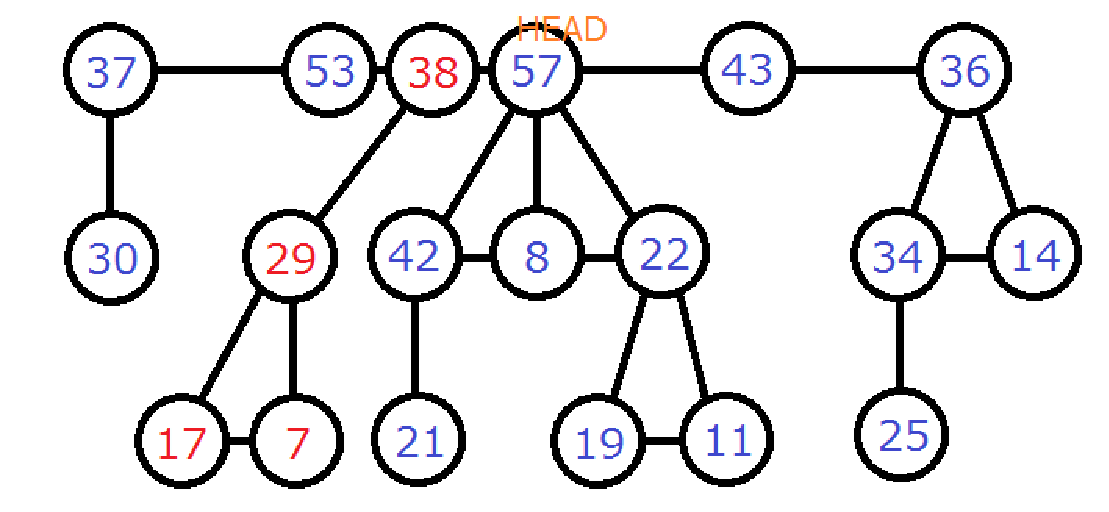
\includegraphics[width=10cm]{image/fibonacci06.pdf}
    }
  \end{exampleblock}
}

\frame{
  \frametitle{pop}
  \begin{block}{pop$(H)$}
    1.  $head[H]$を$H$の根リストから削除する\\
    2.  $head[H]$の子を全て根リストに追加する\\
    3.  $head[H] \leftarrow child[head[H]]$\\
    4.  根リストに含まれる全ての接点の次数が異なるように整理する\\
    5.  根リストから最大値を持つ接点を探し,それをheadにする
  \end{block}
}

\frame{
  \frametitle{pop}
  \begin{exampleblock}{例}
    \center{
      \includegraphics<1>[width=10cm]{image/fibonacci07.pdf}
      \includegraphics<2>[width=10cm]{image/fibonacci08.pdf}
      \includegraphics<3>[width=10cm]{image/fibonacci09.pdf}
      \includegraphics<4>[width=10cm]{image/fibonacci10.pdf}
      \includegraphics<5>[width=10cm]{image/fibonacci11.pdf}
      \includegraphics<6>[width=10cm]{image/fibonacci12.pdf}
      \includegraphics<7>[width=10cm]{image/fibonacci13.pdf}
      \includegraphics<8>[width=10cm]{image/fibonacci14.pdf}
      \includegraphics<9>[width=10cm]{image/fibonacci15.pdf}
      \includegraphics<10>[width=10cm]{image/fibonacci16.pdf}
      \includegraphics<11>[width=10cm]{image/fibonacci17.pdf}
      \includegraphics<12>[width=10cm]{image/fibonacci18.pdf}
    }
  \end{exampleblock}
}

\frame{
  \frametitle{decreaseKey}
  \begin{block}{decreaseKey$(H, x, k)$}
    1.  {\bf If} $k < key[x]$\\
    2. ~~ {\bf Then} error\\
    3.  $key[x] \leftarrow k$\\
    4.  $y \leftarrow parent[x]$\\
    5.  {\bf If} $y \neq$ nil かつ $key[x] > key[y]$\\
    6. ~~ {\bf Then} cut$(H, x)$\\
    7. ~~~~~~~~~~ cascadingCut$(H, y)$\\
    8.  {\bf If} $key[x] > key[head[H]]$\\
    9. ~~ {\bf Then} $head[H] \leftarrow x$
  \end{block}
}

\frame{
  \frametitle{cut, cascadingCut}
  \begin{block}{cut$(H, x)$}
    1.  $y \leftarrow parent[x]$\\
    2.  $y$の子リストから$x$を取り除き,$deg[y] \leftarrow deg[y]-1$\\
    3.  $x$を$H$の値リストに加える\\
    4.  $parent[x] \leftarrow$ nil\\
    5.  $mark[x] \leftarrow$ FALSE
  \end{block}
  \begin{block}{cascadingCut$(H,y)$}
    1.  {\bf If} $parent[y] \neq$ nil\\
    2. ~~ {\bf Then If} $mark[y] =$ FALSE\\
    3. ~~~~~ {\bf Then} $mark[y] \leftarrow$ FALSE\\
    4. ~~~~~ {\bf Else} cut$(H,y)$\\
    5. ~~~~~~~~~~~ cascadingCut$(H,parent[y])$
  \end{block}
}

\frame{
  \frametitle{decreaseKey}
  \begin{exampleblock}{例}
    \center{
      \includegraphics<1>[width=10cm]{image/fibonacci19.pdf}
      \includegraphics<2>[width=10cm]{image/fibonacci20.pdf}
      \includegraphics<3>[width=10cm]{image/fibonacci21.pdf}
      \includegraphics<4>[width=10cm]{image/fibonacci22.pdf}
      \includegraphics<5>[width=10cm]{image/fibonacci23.pdf}
      \includegraphics<6>[width=10cm]{image/fibonacci24.pdf}
      \includegraphics<7>[width=10cm]{image/fibonacci25.pdf}
      \includegraphics<8>[width=10cm]{image/fibonacci26.pdf}
    }
  \end{exampleblock}
}

\frame{
  \frametitle{decreaseKey}
  \begin{alertblock}{decreaseKey}
    接点が親から切り離されるのは,2つの子を失った直後である.
  \end{alertblock}
}

\frame{
  \frametitle{フィボナッチヒープの計算量}
  \begin{block}{Fibonacci Heapの計算量}
    \itemize{
    \item top : $O(1)$でヒープの最大値を求める
    \item push : $O(1)$で$C$の要素$x$を追加する
    \item merge : $O(1)$で2つのヒープを併合する
    \item pop : $O(\log N)$でヒープの最大値をもつ要素を削除する
    \item decrease key : $O(1)$でポインタの先の要素の値を増やす
    \item delete : $O(\log N)$でポインタの先の要素を消去する\\ \\
    }
    ならし計算量(1回あたりの平均)による値\\ \\
    \only<2>{\alert{本当にそんな計算量で実現可能なのか?}} \\
  \end{block}
}

\frame{
  \frametitle{償却計算量}
  \begin{alertblock}{償却計算量}
    操作を複数回行った時の1回あたりのならし計算量
  \end{alertblock}
  \begin{alertblock}{ポテンシャル関数}
    ポテンシャル関数 $\Phi$\\
    $\Phi(H)$ はヒープ $H$ が遅延させている計算回数
  \end{alertblock}
  \center{
    ポテンシャル関数を用いて償却計算量を計算する\\
    ここでは,$\Phi(H) = t(H) + 2m(H)$ とする\\
    $t(H) = |\{x \in V : parent(x)=null\}|$\\
    $m(H) = |\{x \in V : mark[x]=true\}|$\\
  }
}

\frame{
  \begin{exampleblock}{例}
    \center{
      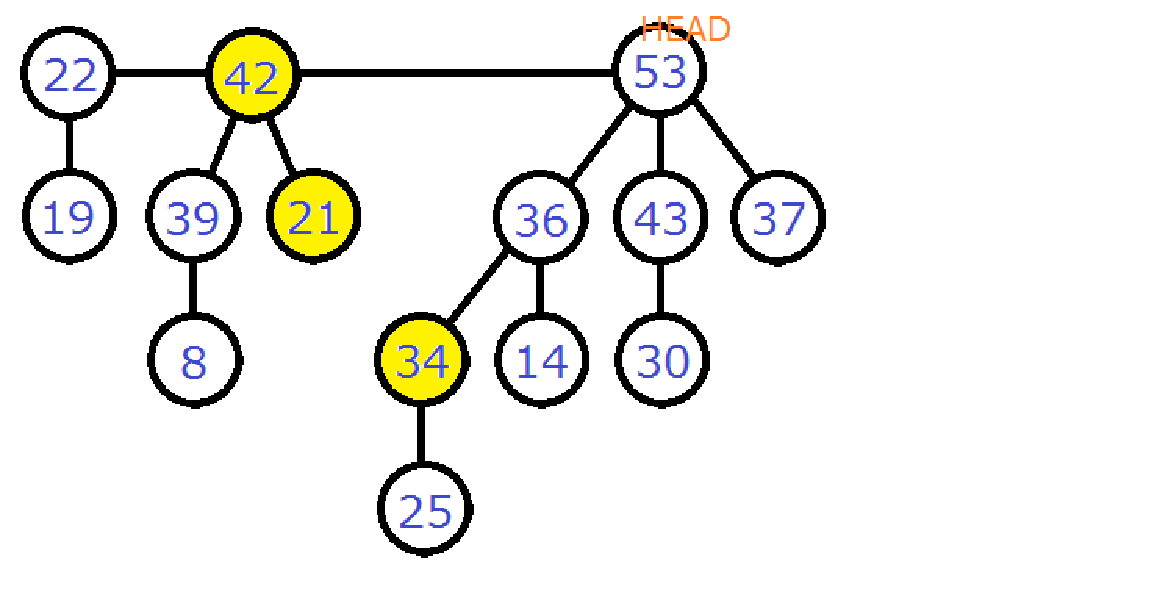
\includegraphics[width=10cm]{image/fibonacci19.pdf}
       \\ \\
      $\Phi(H) = t(H) + 2m(H) = 14 + 2 \cdot 3 = 20$\\
    }
  \end{exampleblock}
}

\frame{
  \frametitle{push}
  \begin{block}{pushの償却計算量}
    $O(1) + (t(H) + 1 +2m(H)) - (t(H) +2m(H)) = O(1)$
  \end{block}
  \begin{exampleblock}{}
    \center{
      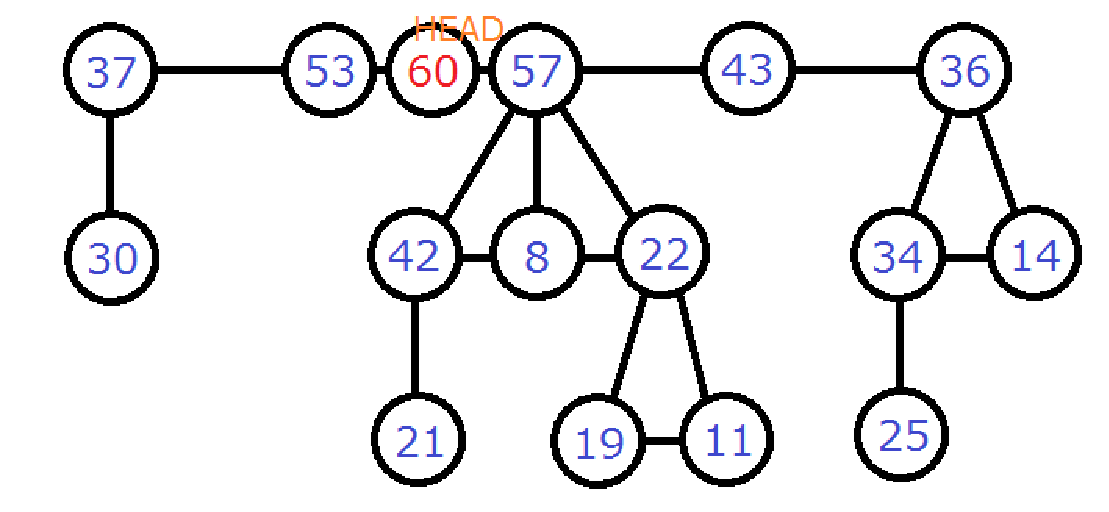
\includegraphics[width=10cm]{image/fibonacci05.pdf}
    }
  \end{exampleblock}
}

\frame{
  \frametitle{merge}
  \begin{block}{mergeの償却計算量}
    ポテンシャルの増加は,\\
    $O(1) + (t(H) + 2m(H)) - (t(H_1) + 2m(H_1)) - (t(H_2) + 2m(H_2))$\\
    ~~~~~~~~~~ $= O(1)$
  \end{block}
  \begin{exampleblock}{}
    \center{
      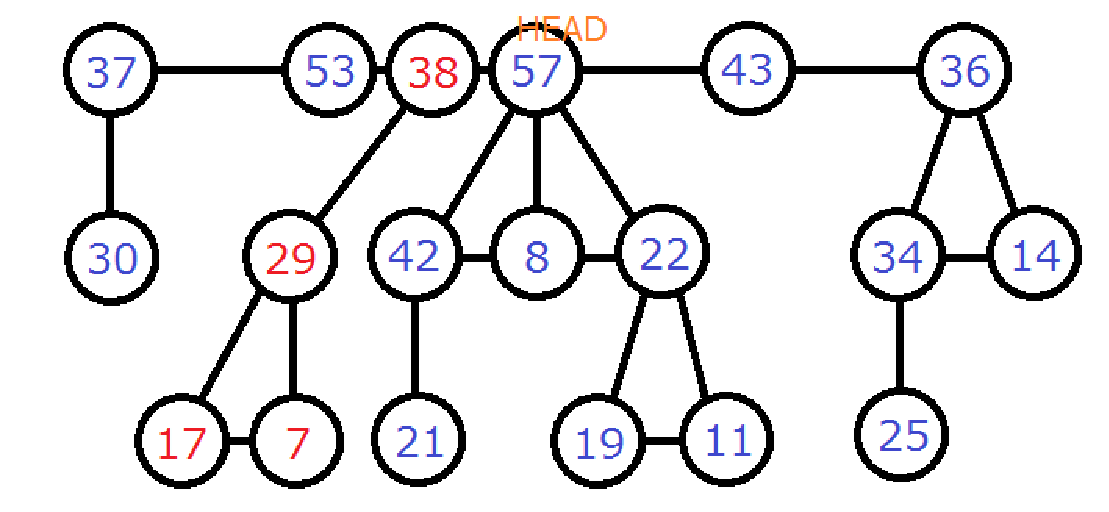
\includegraphics[width=9cm]{image/fibonacci06.pdf}
    }
  \end{exampleblock}
}

\frame{
  \frametitle{decrease key}
  \begin{block}{decrease keyの償却計算量}
    cascading cutが呼び出される回数を$c$回とすると,\\
    $O(c) + ((t(H)+c) + 2(m(H)-c+2)) - (t(H)+2m(H))$\\
    ~~~~~~~~~~~ $= O(c) + 4 - c$\\
    ~~~~~~~~~~~ $= O(1)$
  \end{block}
  \begin{exampleblock}{}
    \center{
      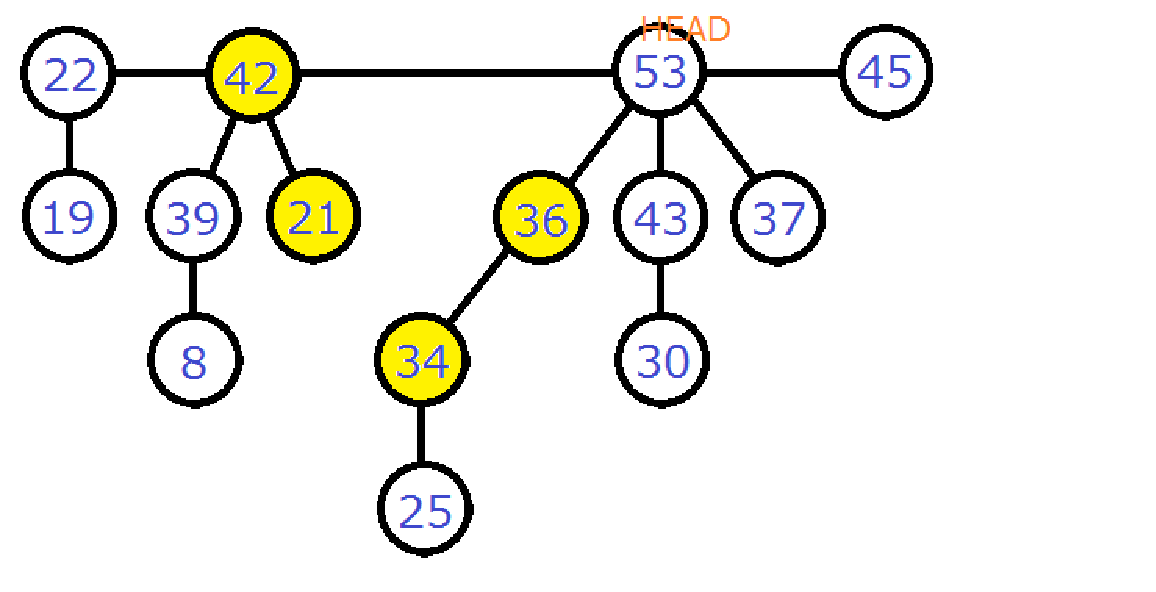
\includegraphics[width=7cm]{image/fibonacci22.pdf}
    }
  \end{exampleblock}
}

\frame{
  \frametitle{pop}
  \begin{block}{popの償却計算量}
    $D(n):=\displaystyle\max_{parent[x]=nil} deg[x]$ として,\\
    $O(D(n) + t(H)) + ((D(n) + 1) + 2m(H)) - (t(H) + 2m(H))$\\
    ~~~~~~~~~~ $= O(D(n)) + O(t(H)) - t(H)$\\
    ~~~~~~~~~~ $= O(D(n))$ \only<2>{$= O(\log N)$}
  \end{block}
  \begin{exampleblock}{}
    \center{
      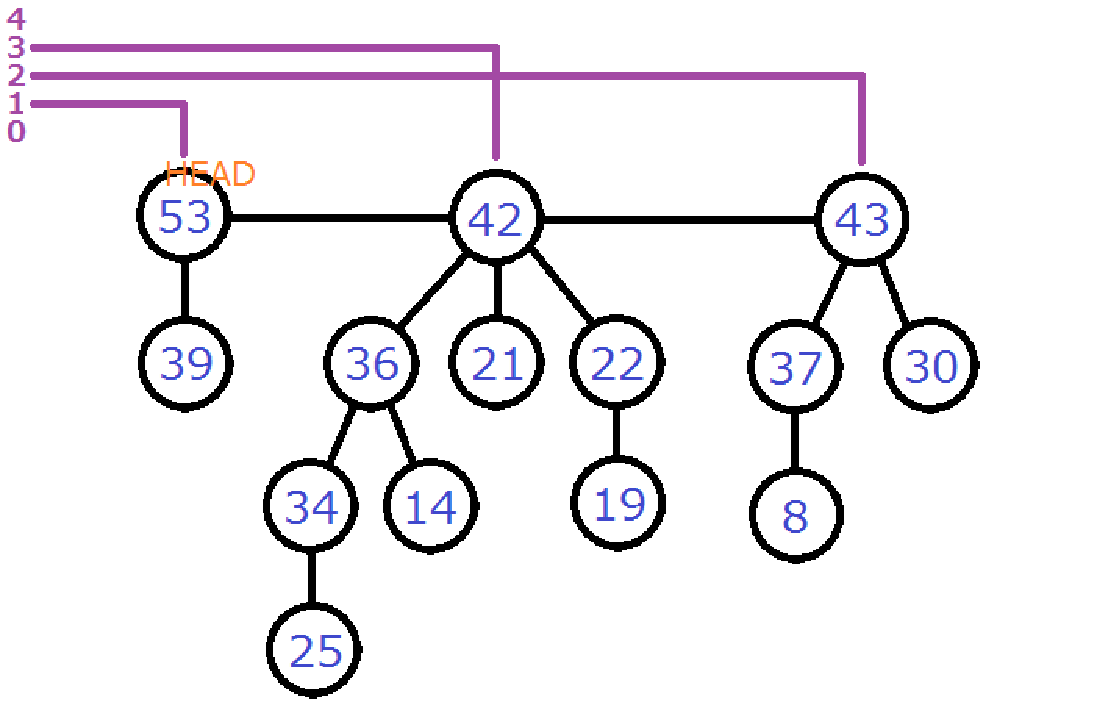
\includegraphics[width=5cm]{image/fibonacci18.pdf}
    }
  \end{exampleblock}
}

\frame{
  \frametitle{最大次数の評価}
  \begin{block}{最大次数の評価}
    $x$を根とした木の接点の数を$size(x)$として,\\
    $size(x) = \Omega(\phi^{deg[x]})$であることを示す.
  \end{block}
  \center{
    \alert{フィボナッチ数を用いた証明!!}\\ \\
    ようやくフィボナッチヒープの名の由来を語る時が来た\\
  }
}

\frame{
  \frametitle{フィボナッチ数の定義}
  \begin{block}{定義}
    $k \in \mathbb{N}$に対して,$k$番目のフィボナッチ数は漸化式
    \begin{eqnarray*}
      F_k =
      \left\{
      \begin{array}{ll}
        0 & (k=0)\\
        1 & (k=1)\\
        F_{k-1}+F_{k-2} & (k\geq 2)\\
      \end{array}
      \right.
    \end{eqnarray*}
    によって定義される.
  \end{block}
}

\frame{
  \frametitle{フィボナッチ数の性質}
  \begin{block}{補題}
    すべての整数$k \geq 0$に対して,
    \[F_{k+2} = 1 + \sum_{i=0}^k F_i\]
  \end{block}
  \begin{block}{補題}
    すべての整数$k \geq 0$に対して,
    \[F_{k+2} \geq \phi ^k\]
    ただし,$\phi$は黄金比であり,$\phi = (1 + \sqrt{5}) / 2$ である.
  \end{block}
  証明略.
}

\frame{
  \frametitle{最大次数の評価}
  \begin{block}{補題}
    $x$をフィボナッチヒープ内の任意の接点とし,$deg[x]=k$とする.
    $x$の子 $y_1, y_2, \cdots, y_k$ が,この順番で$x$に連結
    されたと仮定する.このとき,2以上の整数iに対し,$deg[y_i] \geq i-2$
    が成り立つ.
  \end{block}
  \begin{block}{}
    $y_i$が$x$に連結された時点で,$deg[x]=i$ を満たす.\\
    接点$y_i$が$x$に連結されるのは$deg[x]=deg[y_i]$のときであるので,\\
    $y_i$が$x$に連結された時点で,$deg[y_i] = i-1$ を満たす.\\
    接点は2つの子を失った時点で切断されるはずなので,\\
    $x$に$k$個の接点が連結されている時点で$deg[i] \geq i-2$
  \end{block}
}

\frame{
  \begin{block}{補題}
    $x$をフィボナッチヒープの任意の接点としたとき,\\
    $k=deg[x]$として,$size(x) \geq F_{k+2} \geq \phi ^k$ が成り立つ.\\
  \end{block}
  \begin{block}{}
    $s_k$を$deg[z]=k$となる全ての接点$z$の$size(z)$の最小値とする.\\
    $s_0=1, s_1=2, s_2=3$ は明らか.\\
    3以上の整数$k$について,以下が成り立つ.\\
    \[s_k \geq 2 + \sum_{i=2}^k s_{i-2}\]
  \end{block}
}

\frame{
  \begin{block}{補題}
    \center{
      $k \in \mathbb{N}$ について,$s_k \geq F_{k+2}$
    }
  \end{block}
  \begin{block}{}
    $k$に関する帰納法により証明する.\\
    $k=0$と$k=1$については自明.\\
    $k\geq 2$として,$i \in \{0,1,\cdots ,k-1\}$を仮定したとき,\\
    \begin{eqnarray*}
      s_k &\geq& 2 + \sum_{i=2}^k s_{i-2}\\
          &\geq& 2 + \sum_{i=2}^k F_i\\
          &=& 1 + \sum_{i=0}^k F_i = F_{k+2}
    \end{eqnarray*}
  \end{block}
}

\frame{
  \begin{alertblock}{系}
    $n$接点フィボナッチヒープの接点の最大次数は$O(\log n)$である.\\
  \end{alertblock}
  \begin{alertblock}{}
    補題より,
    \[size(x) \geq s_k \geq F_{k+2} \geq \phi ^k\]
    を得る.つまり,$n \geq \phi ^k$であるので,$k \leq \log_{\phi} n$である.\\ \\
    よって,最大次数$D(n)=O(\log n)$である.
  \end{alertblock}
}
